\documentclass{zc-ust-hw}

\usepackage{lipsum}

\name{SalahDin Ahmed Salh Rezk}
\id{202201079}
\course{CIE 212 Project}
\assignment{Design and Implementation of a Rectifier Circuit\\for 220V AC to 5V DC Conversion}

\begin{document}

\maketitle
\tableofcontents

\begin{abstract}
This project aims to design and implement a rectifier circuit for converting
220V AC to 5V DC. The circuit consists of a step-down transformer, a bridge
rectifier, a filtering capacitor, and a voltage regulator. The theoretical
calculations and practical testing were conducted to verify the circuit's
performance and efficiency. The design ensures that the ripple voltage does not
exceed 2\% of the DC output.
\end{abstract}

\newpage

\section{Theory}
Rectifiers are classified into different types based on their configuration and
operation, such as half-wave rectifiers, full-wave rectifiers, and bridge
rectifiers. Each type has distinct characteristics and efficiency levels.

\subsection{Step-Down Transformer}
A step-down transformer reduces the 220V AC to a lower AC voltage. The turns ratio \( n \) of the transformer is given by:
\[
n = \frac{V_{\text{primary}}}{V_{\text{secondary}}}
\]
For a primary voltage of 220V and a desired secondary voltage of 12V:
\[
n = \frac{220}{12} \approx 18.33
\]

Alternatively, transformers can be represented as conductance ratios:

\[
\frac{V_{\text{primary}}}{V_{\text{secondary}}} = \left( \frac{N_{\text{primary}}}{N_{\text{secondary}}} \right)^2
\] 

which is crucial for our simulation.

\subsection{Bridge Rectifier}
A bridge rectifier, consisting of four diodes, provides a full-wave rectified output. The DC output voltage \( V_{\text{DC}} \) can be approximated by:
\[
V_{\text{DC}} \approx \frac{2V_{\text{secondary}}}{\pi}
\]
For a 12V AC secondary:
\[
V_{\text{DC}} \approx \frac{2 \times 12}{\pi} \approx 7.64V
\]

\subsection{Filtering}

To smooth the pulsating DC output from the bridge rectifier, a capacitor filter is used. The ripple voltage \( V_{\text{ripple}} \) is estimated by:
\[
V_{\text{ripple}} = \frac{V_{\text{DC}}}{f \cdot R_{\text{load}} \cdot C}
\]
where \( V_{\text{DC}} \) is the DC output voltage, \( f \) is the frequency (100Hz for full-wave rectified output), \( R_{\text{load}} \) is the load resistance, and \( C \) is the capacitance.

To achieve a ripple voltage of no more than 2\% of the 5V output:
\[
V_{\text{ripple}} \leq 0.02 \times 5 = 0.1V
\]
Rearranging the formula to solve for \( C \):
\[
C \geq \frac{V_{\text{DC}}}{f \cdot R_{\text{load}} \cdot V_{\text{ripple}}}
\]
Assuming \( V_{\text{DC}} = 7.64V \), \( f = 100 \text{Hz} \), and a load resistance \( R_{\text{load}} = 15 k\Omega \):
\[
C \geq \frac{7.64}{100 \times 5 \times 0.1} \approx 1000 \mu F
\]

\subsection{Voltage Regulation}

A voltage regulator, such as the 7805, ensures a stable 5V DC output. The
regulator smooths out any remaining fluctuations in the voltage. It takes the
input voltage and adjusts it to the desired output voltage. The 7805 regulator
is a type of linear regulator that uses a series pass transistor to maintain a
constant output voltage. It is commonly used in electronic circuits to provide
a stable 5V supply.

An alternative is to use a Zener diode to regulate the voltage, but it is less
efficient than a voltage regulator.

The zener diode is a type of diode that allows current to flow in the forward
direction like a normal diode, but it also permits it to flow in the reverse
direction when the voltage is above a certain value. This is known as the zener
voltage.

The 7805 regulator is more efficient and reliable than a Zener diode, making it
the preferred choice for voltage regulation in this project. However, the Zener
diode can be used as they are cheaper and easier to find.

\section{Design and Implementation}

The design process includes selecting a step-down transformer with a primary
voltage of 220V and a secondary voltage of 12V. A bridge rectifier, constructed
using four diodes (e.g., 1N4007), is connected to the AC output of the
transformer to convert it to DC. To filter the rectified output, a capacitor
with a suitable value is chosen; for instance, with a load current of 1A and a
ripple voltage of 0.1V, a capacitance of at least 10000 µF is required.
Finally, the filtered DC output is fed into a 7805 voltage regulator to achieve
a stable 5V DC output.

\subsection{Simulation}

The circuit is then implemented using LTspice to simulate its performance and
verify the theoretical calculations. The output voltage, ripple voltage, and
efficiency are measured and analyzed to ensure the circuit's reliability and
effectiveness. Figure~\ref{fig:ltspice-circuit} shows the rectifier circuit
implemented on LTspice. A special Zener diode was used to regulate the voltage
in this simulation because it is what was available in stock. 

\begin{figure}[h]
  \begin{center}
    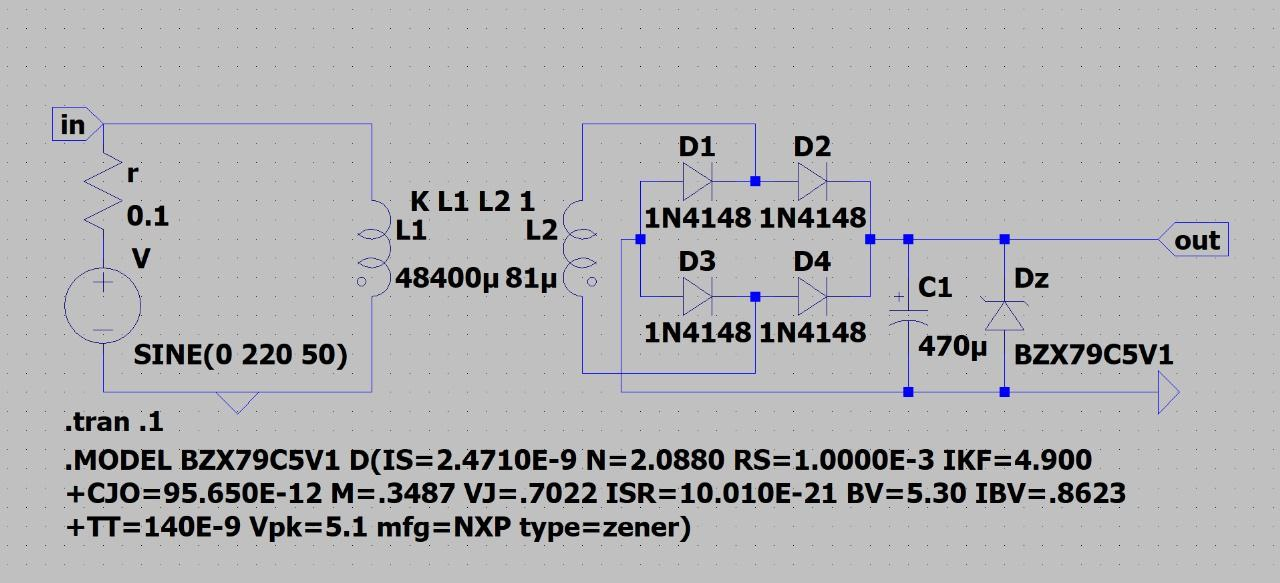
\includegraphics[width=0.75\textwidth]{figures/photo_2024-05-24_00-16-34.jpg}
  \end{center}
  \caption{Rectifier Circuit on LTspice}
  \label{fig:ltspice-circuit}
\end{figure}

\begin{figure}[h]
  \begin{center}
    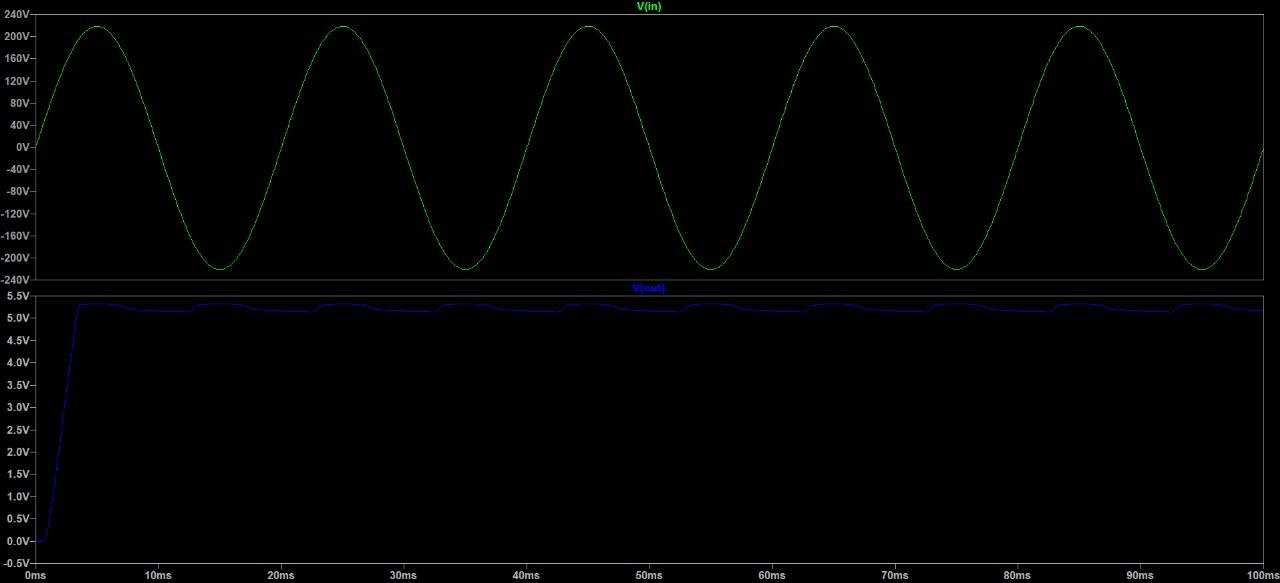
\includegraphics[width=0.75\textwidth]{figures/photo_2024-05-24_00-16-35.jpg}
  \end{center}
  \caption{Graph of the output voltage}
  \label{fig:ltspice-circuit}
\end{figure}

\subsection{Hardware (Bonus)}

This section was done with collaboration with Abdelrahman Magdy and Khaled Mahmoud.

The circuit is then implemented on a breadboard using the actual components. The
transformer, diodes, capacitor, and voltage regulator are connected as per the
design. The output voltage and ripple voltage are measured using an oscilloscope
to verify the circuit's performance. The hardware implementation ensures that
the rectifier circuit can be used in practical applications. Figure~\ref{fig:breadboard-circuit} shows the rectifier circuit implemented on a breadboard, and Figure~\ref{fig:oscilloscope-measurement} shows the oscilloscope measurement of the output voltage.

\begin{figure}[h]
  \begin{center}
    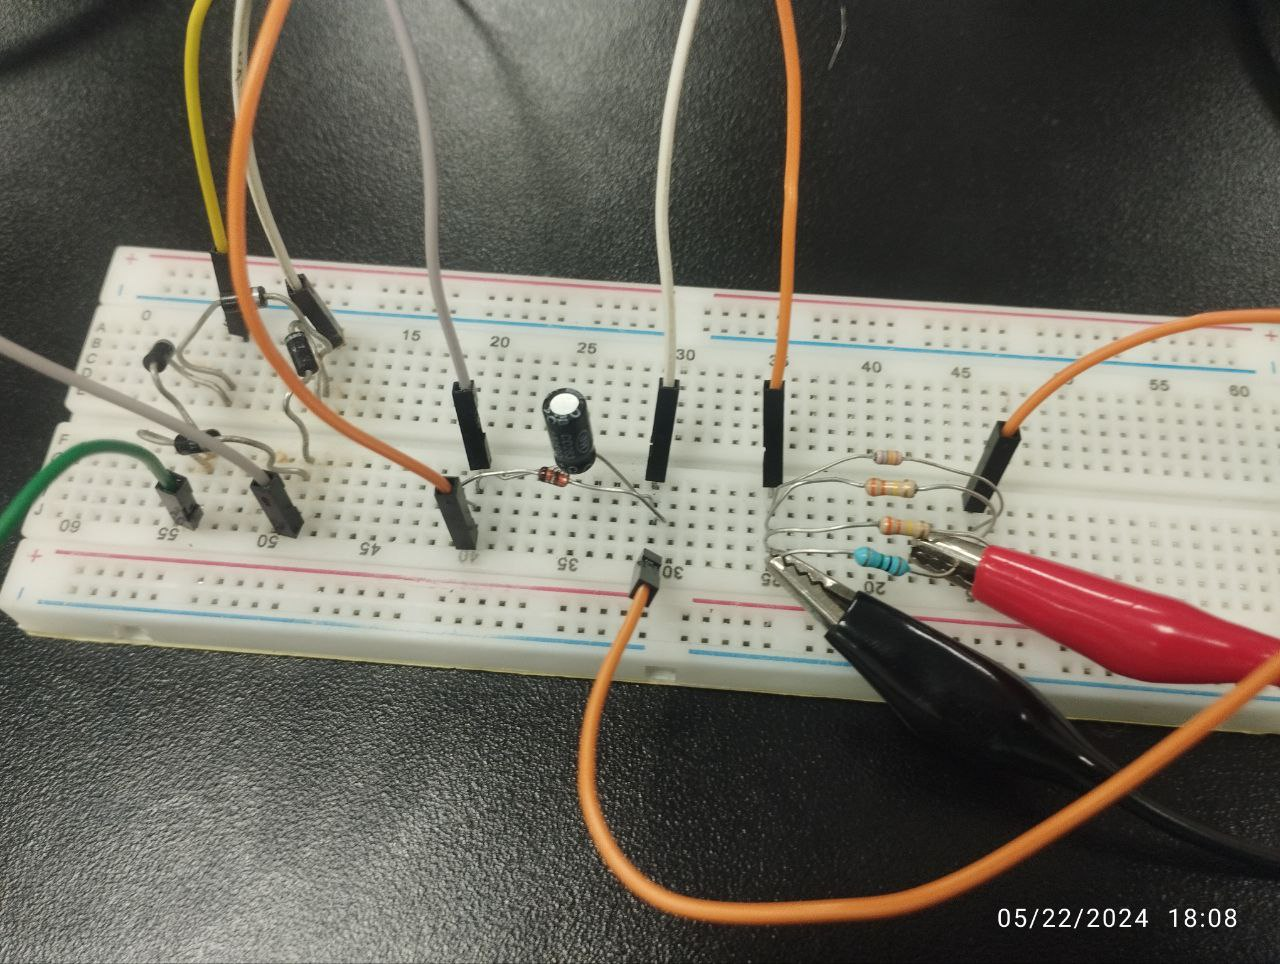
\includegraphics[width=0.75\textwidth]{figures/photo_2024-05-24_00-16-43.jpg}
  \end{center}
  \caption{Rectifier Circuit on Breadboard}
  \label{fig:breadboard-circuit}
\end{figure}

\begin{figure}[H]
  \begin{center}
    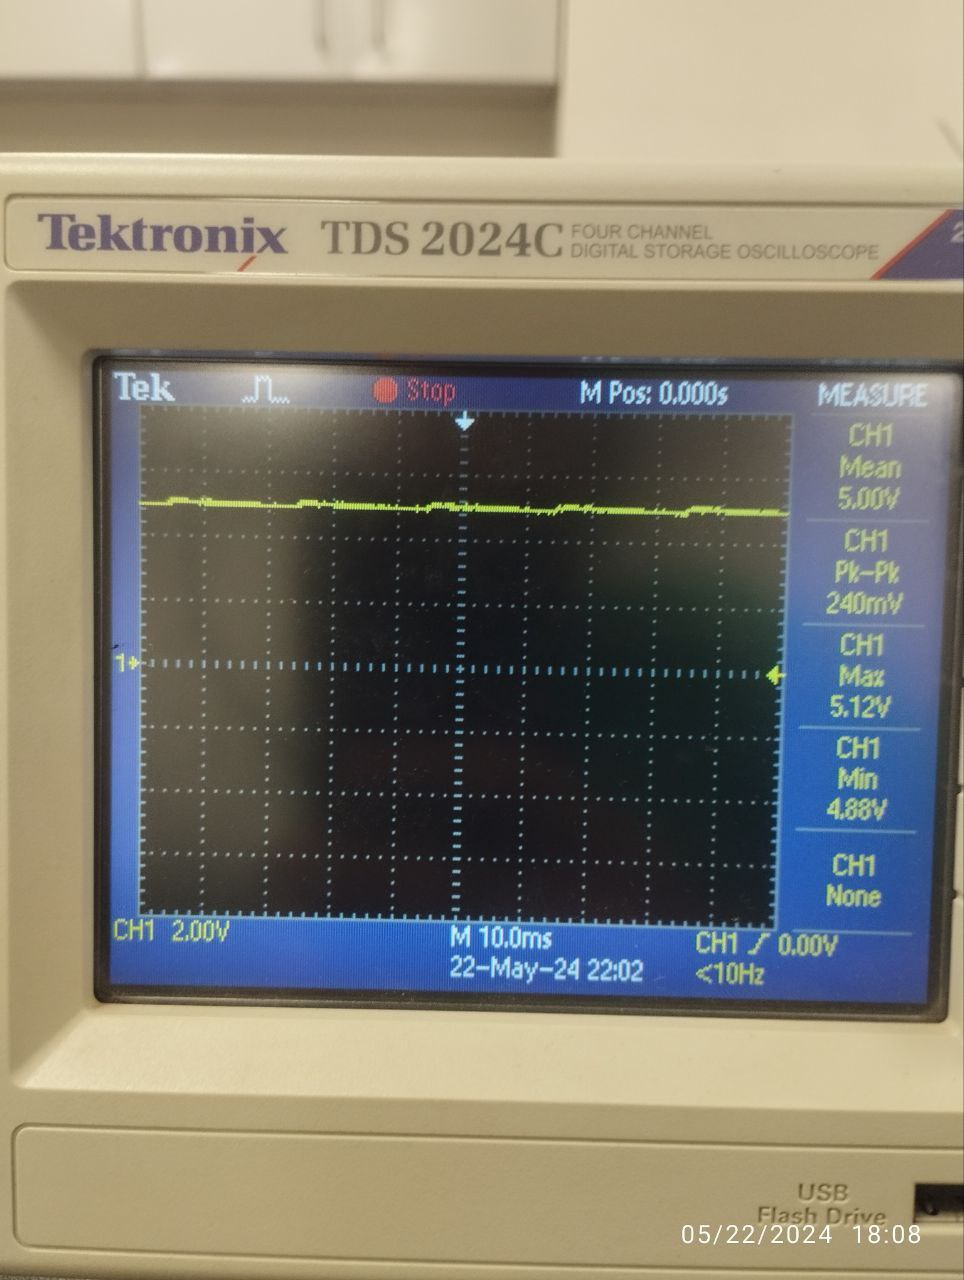
\includegraphics[width=0.5\textwidth]{figures/photo_2024-05-24_00-16-45.jpg}
  \end{center}
  \caption{Oscilloscope Measurement of the Output Voltage}
  \label{fig:oscilloscope-measurement}
\end{figure}

We also used a regulator to regulate the voltage. The regulator is a 7805
voltage regulator that provides a stable 5V output. The regulator is connected
to the output of the rectifier circuit to ensure a constant voltage supply. The
regulator is essential for maintaining a stable voltage output, which is
crucial for electronic devices.

With the regulator, we used the circuit to power an LED to demonstrate its practical
application. The rectifier circuit successfully converted 220V AC to a stable 5V
DC output, which was used to light up the LED. See Figure~\ref{fig:led-lighting}.

\begin{figure}[h]
  \begin{center}
    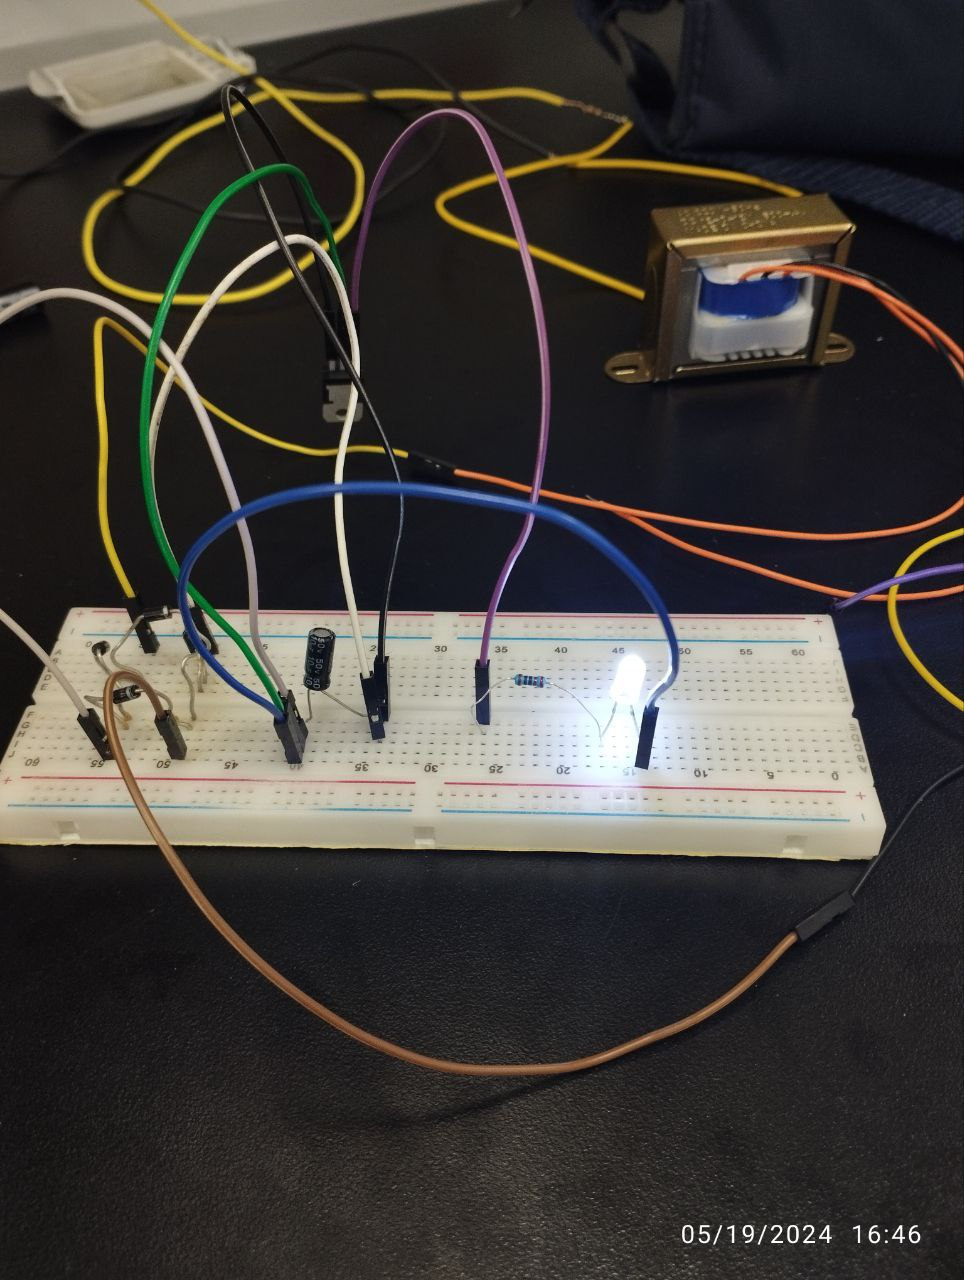
\includegraphics[width=0.55\textwidth]{figures/photo_2024-05-24_00-16-41.jpg}
  \end{center}
  \caption{LED Powered by the Rectifier Circuit}
  \label{fig:led-lighting}
\end{figure}

\section{Results}
The rectifier circuit was tested under different load
conditions. The output voltage and current were measured and analyzed to ensure
the circuit's efficiency and reliability. The measured DC output voltage was
consistently around 5V, confirming the effectiveness of the voltage regulator.
The ripple voltage was within the 2\% acceptable range, ensuring a stable DC
supply for electronic devices.

\section{Conclusion}
This project provided hands-on experience in designing and implementing
rectifier circuits. The step-down transformer, bridge rectifier, capacitor
filter, and voltage regulator effectively converted 220V AC to a stable 5V DC
with a ripple voltage not exceeding 2\%. Understanding the different types of
rectifiers and their applications is crucial for various electronic projects.

\end{document}
